\documentclass[a4paper,12pt]{article}
\usepackage{../packages/coursCollege}
\newcommand{\Chapitre}{Calcul différentiel}
\renewcommand{\path}{../}
\usepackage[    %backend=biber, 
    natbib=true,
    style=numeric,
    sorting=none]{biblatex}  % Load biblatex for bibliography handling
\addbibresource{biblio-der.bib}  
\renewcommand\refname{Sources}
\renewcommand{\cours}{3MA1~--~EG~--~ns~--~2025-2026}
\usepackage{subcaption}
% Définition des couleurs
\definecolor{functioncolor}{RGB}{220,50,47}
\definecolor{tangentcolor}{RGB}{220,50,47}
\definecolor{secantcolor}{RGB}{38,139,210}
\definecolor{pointcolor}{RGB}{220,50,47}

\begin{document}
\tocloftpagestyle{fancy}
% Reduce space between section entries
\setlength{\cftbeforesecskip}{2pt}

% Reduce indentation for section entries
\setlength{\cftsecindent}{1em}
\begin{center}
{\bfseries \Huge Chapitre 2~: \\Calcul différentiel}
\vspace{1cm}

\begin{tikzpicture}
% Background image
\node[inner sep=0] at (0,0) {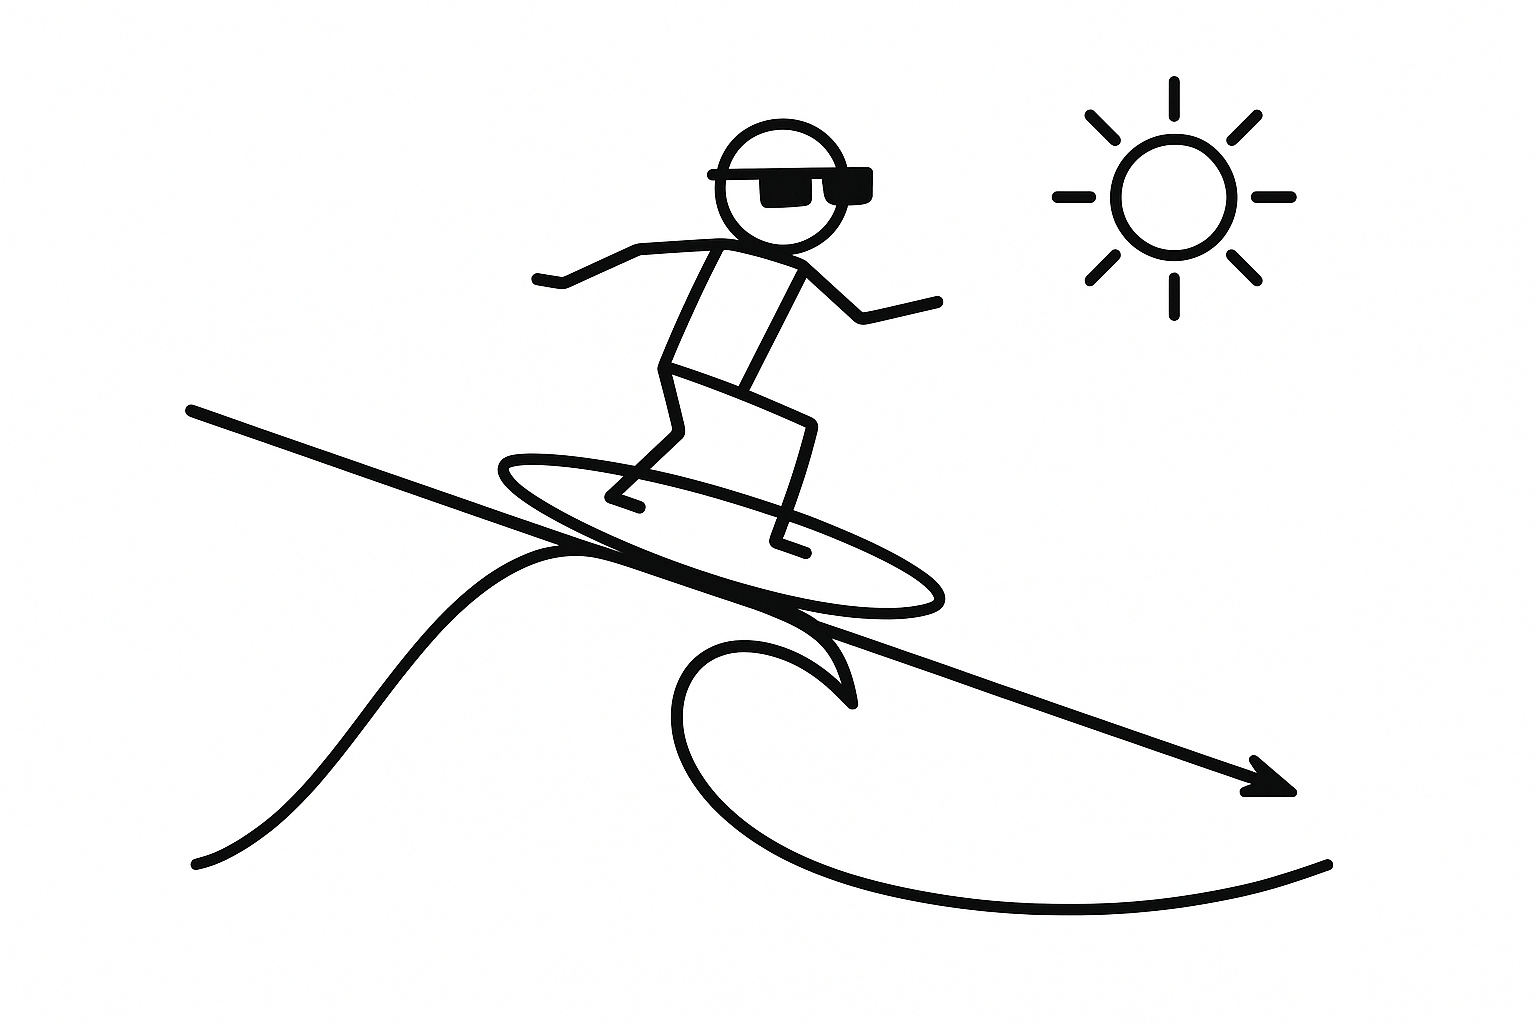
\includegraphics[width=15cm]{../medias/3M/derivation/intro}};
\end{tikzpicture}
\end{center}\vspace{-1cm}
\tableofcontents

\newpage
\section{La dérivée}

\subsection{Introduction : La tangente à une courbe en un point}

Nous commençons avec une fonction $f$, et sur le graphique nous choisissons un point $(x, f(x))$ (c.f. Figure~\ref{fig:der1}). Quelle droite, s'il y en a une, devrait être appelée tangente au graphique en ce point~? Et comment déterminer son équation~?

\begin{figure}[h]
\centering
\begin{subfigure}[c]{0.4\textwidth}
	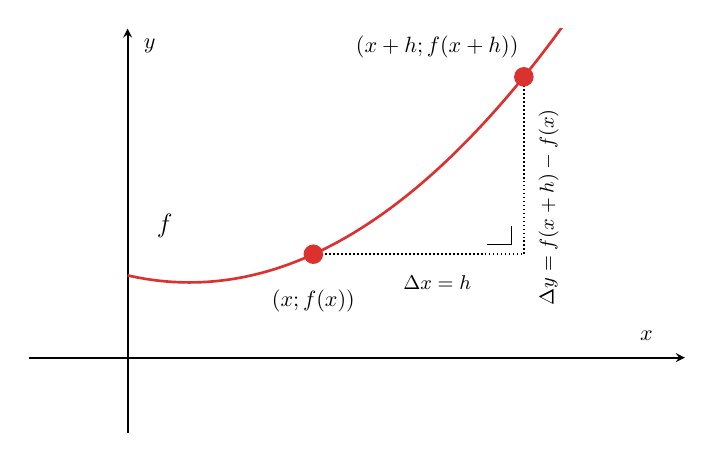
\begin{tikzpicture}[scale=0.8]
\begin{axis}[
    width=12cm,
    height=8cm,
    axis lines=middle,
    xlabel={$x$},
    ylabel={$y$},
    every axis x label/.style={at={(ticklabel* cs:0.92)}, anchor=west, yshift=10pt},
    every axis y label/.style={at={(ticklabel* cs:0.92)}, anchor=south, xshift=10pt},
    xmin=-0.8, xmax=4.5,
    ymin=-0.8, ymax=3.5,
    xtick=\empty,
    ytick=\empty,
    samples=200,
    axis line style={thick},
    every axis plot/.append style={thick},
]

% Fonction f(x) = 0.3*(x-0.5)^2 + 0.8
\addplot[
    domain=0:4,
    very thick,
    color=functioncolor,
] {0.3*(x-0.5)^2 + 0.8};

% Point (x, f(x))
\addplot[
    mark=*,
    mark size=4pt,
    color=pointcolor,
    only marks,
] coordinates {(1.5, 0.3+0.8)};
% Point (x, f(x))
\addplot[
    mark=*,
    mark size=4pt,
    color=pointcolor,
    only marks,
] coordinates {(3.2, 0.3*2.7*2.7+0.8)};

% Label du point avec fond blanc pour la lisibilité
\node[fill=white, inner sep=2pt] at (axis cs:1.5, 0.6) {$(x;f(x))$};

% Label de la fonction avec fond blanc
\node[fill=white, inner sep=2pt, font=\large] at (axis cs:0.3, 1.4) {$f$};
% Triangle de pente
% Ligne horizontale (Delta x)
\draw[thick, color=black, densely dotted] (axis cs:1.5,1.1) -- (axis cs:3.2,1.1);
% Ligne verticale (Delta y)  
\draw[thick, color=black, densely dotted] (axis cs:3.2,1.1) -- (axis cs:3.2,2.987);

% Angle droit
\draw[color=black] (axis cs:2.9,1.2) -- (axis cs:3.1,1.2) -- (axis cs:3.1,1.4);

% Labels des points
\node at (axis cs:2.5, 3.3) {$(x + h; f(x + h))$};

% Labels du triangle
\node[font=\small] at (axis cs:2.5, 0.8) {{$\Delta x = h$}};
\node[rotate=90, font=\small] at (axis cs:3.4, 1.6) {{$\Delta y = f(x+h) - f(x)$}};
\end{axis}
\end{tikzpicture}
\subcaption{Un point sur le graphe de $f$}
\end{subfigure}
\hfill
\begin{subfigure}[c]{0.48\textwidth}
	\centering
	\qrcode[height=3cm]{https://derivee.gemaths.net}
	\subcaption{Une appliquette pour visualiser différentes situations}
\end{subfigure}
\caption{Introduction à notion de dérivée}
\label{fig:der1}
\end{figure}

Pour répondre à cette question, nous choisissons un petit nombre $h \neq 0$ et sur le graphique marquons le point $(x + h, f(x + h))$. Maintenant nous traçons la droite sécante qui passe par ces deux points. La situation est illustrée dans la Figure~3.1.2 en prenant des valeurs de $h>0$.

\begin{figure}[h]
\centering
\begin{subfigure}[b]{0.4\textwidth}
\centering
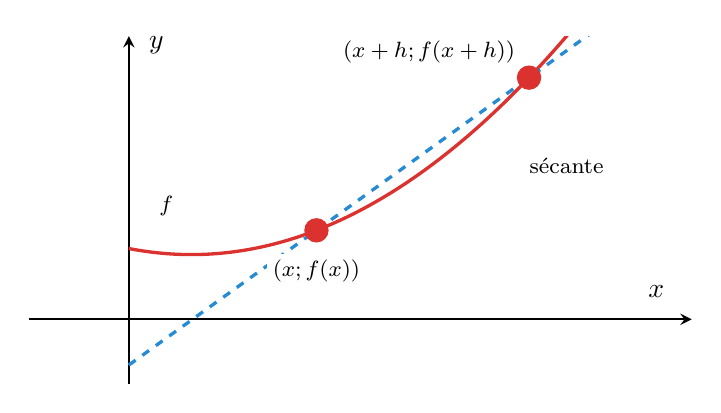
\begin{tikzpicture}
\begin{axis}[
    width=10cm,
    height=6cm,
    axis lines=middle,
    xlabel={$x$},
    ylabel={$y$},
    every axis x label/.style={at={(ticklabel* cs:0.92)}, anchor=west, yshift=10pt},
    every axis y label/.style={at={(ticklabel* cs:0.92)}, anchor=south, xshift=10pt},
    xmin=-0.8, xmax=4.5,
    ymin=-0.8, ymax=3.5,
    xtick=\empty,
    ytick=\empty,
    samples=200,
    axis line style={thick},
    every axis plot/.append style={thick},
]

% Fonction f(x) = 0.3*(x-0.5)^2 + 0.8
\addplot[
    domain=0:4,
    very thick,
    color=functioncolor,
] {0.3*(x-0.5)^2 + 0.8};

% Fonction f(x) = 0.3*(x-0.5)^2 + 0.8
\addplot[
    domain=0:4,
    very thick,
    color=secantcolor,
    dashed
] {1.11*x - 0.565};

% Point (x, f(x))
\addplot[
    mark=*,
    mark size=4pt,
    color=pointcolor,
    only marks,
] coordinates {(1.5, 0.3+0.8)};

% Point (x, f(x))
\addplot[
    mark=*,
    mark size=4pt,
    color=pointcolor,
    only marks,
] coordinates {(3.2, 0.3*2.7*2.7+0.8)};

% Label du point avec fond blanc pour la lisibilité
\node[fill=white, inner sep=2pt, font=\footnotesize] at (axis cs:1.5, 0.6) {$(x;f(x))$};
\node[fill=white, inner sep=2pt, font=\footnotesize] at (axis cs:2.4, 3.3) {$(x+h;f(x+h))$};

% Label de la fonction avec fond blanc
\node[fill=white, inner sep=2pt, font=\footnotesize] at (axis cs:0.3, 1.4) {$f$};
\node[fill=white, inner sep=2pt, font=\footnotesize] at (axis cs:3.5, 1.9) {sécante};

\end{axis}
\end{tikzpicture}
\subcaption*{$h=0,4$}
\end{subfigure}
\hfill
\begin{subfigure}[b]{0.4\textwidth}
\centering
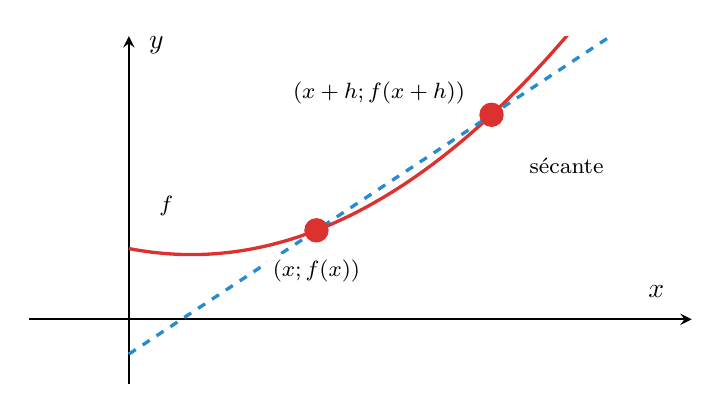
\begin{tikzpicture}
\begin{axis}[
    width=10cm,
    height=6cm,
    axis lines=middle,
    xlabel={$x$},
    ylabel={$y$},
    every axis x label/.style={at={(ticklabel* cs:0.92)}, anchor=west, yshift=10pt},
    every axis y label/.style={at={(ticklabel* cs:0.92)}, anchor=south, xshift=10pt},
    xmin=-0.8, xmax=4.5,
    ymin=-0.8, ymax=3.5,
    xtick=\empty,
    ytick=\empty,
    samples=200,
    axis line style={thick},
    every axis plot/.append style={thick},
]

% Fonction f(x) = 0.3*(x-0.5)^2 + 0.8
\addplot[
    domain=0:4,
    very thick,
    color=functioncolor,
] {0.3*(x-0.5)^2 + 0.8};

% Fonction f(x) = 0.3*(x-0.5)^2 + 0.8
\addplot[
    domain=0:4,
    very thick,
    color=secantcolor,
    dashed
] {1.02*x - 0.43};

% Point (x, f(x))
\addplot[
    mark=*,
    mark size=4pt,
    color=pointcolor,
    only marks,
] coordinates {(1.5, 0.3+0.8)};

% Point (x, f(x))
\addplot[
    mark=*,
    mark size=4pt,
    color=pointcolor,
    only marks,
] coordinates {(2.9, 0.3*2.4*2.4+0.8)};

% Label du point avec fond blanc pour la lisibilité
\node[fill=white, inner sep=2pt, font=\footnotesize] at (axis cs:1.5, 0.6) {$(x;f(x))$};
\node[fill=white, inner sep=2pt, font=\footnotesize] at (axis cs:2, 2.8) {$(x+h;f(x+h))$};

% Label de la fonction avec fond blanc
\node[fill=white, inner sep=2pt, font=\footnotesize] at (axis cs:0.3, 1.4) {$f$};
\node[fill=white, inner sep=2pt, font=\footnotesize] at (axis cs:3.5, 1.9) {sécante};

\end{axis}
\end{tikzpicture}
\subcaption*{$h=0,3$}
\end{subfigure}

\centering
\begin{subfigure}[b]{0.4\textwidth}
\centering
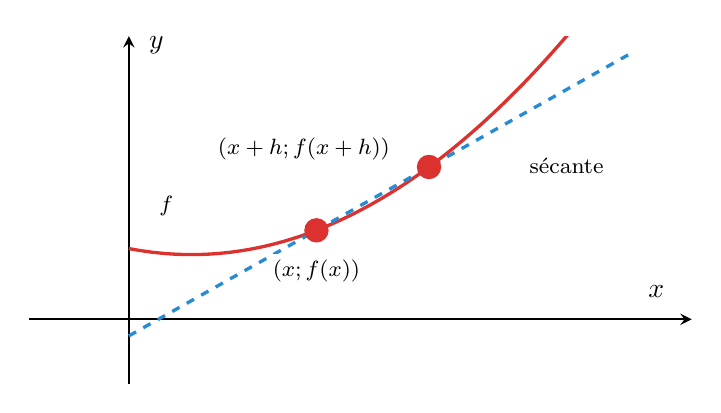
\begin{tikzpicture}
\begin{axis}[
    width=10cm,
    height=6cm,
    axis lines=middle,
    xlabel={$x$},
    ylabel={$y$},
    every axis x label/.style={at={(ticklabel* cs:0.92)}, anchor=west, yshift=10pt},
    every axis y label/.style={at={(ticklabel* cs:0.92)}, anchor=south, xshift=10pt},
    xmin=-0.8, xmax=4.5,
    ymin=-0.8, ymax=3.5,
    xtick=\empty,
    ytick=\empty,
    samples=200,
    axis line style={thick},
    every axis plot/.append style={thick},
]

% Fonction f(x) = 0.3*(x-0.5)^2 + 0.8
\addplot[
    domain=0:4,
    very thick,
    color=functioncolor,
] {0.3*(x-0.5)^2 + 0.8};

% Fonction f(x) = 0.3*(x-0.5)^2 + 0.8
\addplot[
    domain=0:4,
    very thick,
    color=secantcolor,
    dashed
] {0.87*x-0.205};

% Point (x, f(x))
\addplot[
    mark=*,
    mark size=4pt,
    color=pointcolor,
    only marks,
] coordinates {(1.5, 0.3+0.8)};

% Point (x, f(x))
\addplot[
    mark=*,
    mark size=4pt,
    color=pointcolor,
    only marks,
] coordinates {(2.4, 0.3*1.9*1.9+0.8)};

% Label du point avec fond blanc pour la lisibilité
\node[fill=white, inner sep=2pt, font=\footnotesize] at (axis cs:1.5, 0.6) {$(x;f(x))$};
\node[fill=white, inner sep=2pt, font=\footnotesize] at (axis cs:1.4, 2.1) {$(x+h;f(x+h))$};

% Label de la fonction avec fond blanc
\node[fill=white, inner sep=2pt, font=\footnotesize] at (axis cs:0.3, 1.4) {$f$};
\node[fill=white, inner sep=2pt, font=\footnotesize] at (axis cs:3.5, 1.9) {sécante};

\end{axis}
\end{tikzpicture}
\subcaption*{$h=0,15$}
\end{subfigure}
\hfill
\begin{subfigure}[b]{0.4\textwidth}
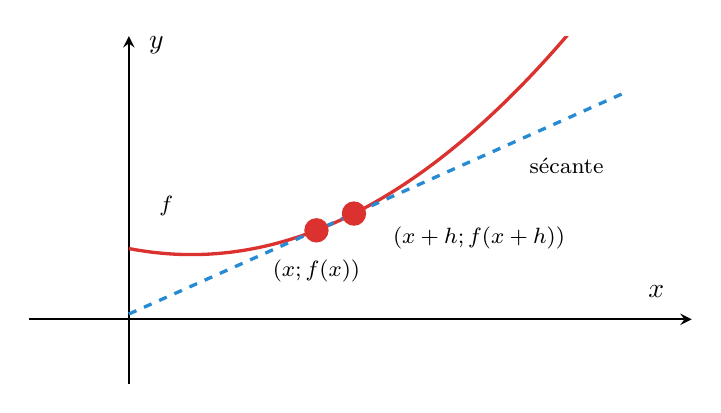
\begin{tikzpicture}
\begin{axis}[
    width=10cm,
    height=6cm,
    axis lines=middle,
    xlabel={$x$},
    ylabel={$y$},
    every axis x label/.style={at={(ticklabel* cs:0.92)}, anchor=west, yshift=10pt},
    every axis y label/.style={at={(ticklabel* cs:0.92)}, anchor=south, xshift=10pt},
    xmin=-0.8, xmax=4.5,
    ymin=-0.8, ymax=3.5,
    xtick=\empty,
    ytick=\empty,
    samples=200,
    axis line style={thick},
    every axis plot/.append style={thick},
]

% Fonction f(x) = 0.3*(x-0.5)^2 + 0.8
\addplot[
    domain=0:4,
    very thick,
    color=functioncolor,
] {0.3*(x-0.5)^2 + 0.8};

% Fonction f(x) = 0.3*(x-0.5)^2 + 0.8
\addplot[
    domain=0:4,
    very thick,
    color=secantcolor,
    dashed
] {0.69*x+0.065};

% Point (x, f(x))
\addplot[
    mark=*,
    mark size=4pt,
    color=pointcolor,
    only marks,
] coordinates {(1.5, 0.3+0.8)};

% Point (x, f(x))
\addplot[
    mark=*,
    mark size=4pt,
    color=pointcolor,
    only marks,
] coordinates {(1.8, 0.3*1.3*1.3+0.8)};

% Label du point avec fond blanc pour la lisibilité
\node[fill=white, inner sep=2pt, font=\footnotesize] at (axis cs:1.5, 0.6) {$(x;f(x))$};
\node[fill=white, inner sep=2pt, font=\footnotesize] at (axis cs:2.8, 1) {$(x+h;f(x+h))$};

% Label de la fonction avec fond blanc
\node[fill=white, inner sep=2pt, font=\footnotesize] at (axis cs:0.3, 1.4) {$f$};
\node[fill=white, inner sep=2pt, font=\footnotesize] at (axis cs:3.5, 1.9) {sécante};

\end{axis}
\end{tikzpicture}
\subcaption*{$h=0,05$}
\end{subfigure}
\caption{Construction de la dérivée}
\end{figure}
\hfill

\vspace{0.5cm}

Lorsque $h$ tend vers zéro (une limite!), la droite sécante tend (si la limite existe) vers « la tangente de $f$ au point $(x, f(x))$ ».

Puisque les droites sécantes ont une pente de la forme
\begin{equation}
\frac{f(x + h) - f(x)}{h},
\end{equation}

nous admettons que la position limite de ces sécantes ont une pente
\begin{equation}
\lim_{h \to 0} \frac{f(x + h) - f(x)}{h}.
\end{equation}

Nous commençons l'étude systématique de telles limites, ce que les mathématiciens appellent le calcul différentiel.

\begin{center}
\qrwithlabel{Voyage au pays de maths -- Flâneries infinitésimales}{https://www.arte.tv/fr/videos/097454-003-A/voyages-au-pays-des-maths/}
\end{center}
\subsection{Définitions et exemples}
\begin{definition}
	\tcblower
	Une fonction est dite dérivable en $x$ ssi la limite
	\begin{equation}
		\lim_{h\to0}\dfrac{ f(x+h)-f(x)}{h} \text{ existe et est finie.}
		\label{def:der}
		\tag{$\star$}
	\end{equation}
	Si cette limite existe, on l'appelle la dérivée de $f$ en $x$ et on la note $f'(x)$.  
\end{definition}
\begin{definition}
	\tcblower
On interprète $f'(x)$ comme la pente de la courbe $f$ au point $(x;f(x))$. La droite qui passe par ce point et qui a cette pente s'appelle la tangente à $f$ au point $(x;f(x))$. 
\end{definition}
\begin{remarque}
	\tcblower
	Certaines fonctions sont dérivable sur $\mathbb{R}$, d'autres seulement sur un intervalle donné ou en certains points.
\end{remarque}
\begin{remarque}[label=rem:derdg]
	\tcblower 
On parle de dérivée à droite ou dérivée à gauche si au lieu de prendre la limite birectionnelle dans (\ref{def:der}), on prend la limite à droite ou à gauche.
\end{remarque}
\begin{autre}
	\tcblower
	Commençons par calculer quelques dérivées à l'aide de la définition.
\end{autre}

\begin{exemple}
	\tcblower
	Calcul de la dérivée de $f(x)=x^2$. 

	On part de la définition de la dérivée, on a 

\medskip

$\begin{aligned}
	\dfrac{f(x+h) - f(x)}{h} &= \dfrac{(x+h)^2 - x^2}{h}\\
				 &=\dfrac{(x+h)^2 - x^2}{h}\\
				 &=\dfrac{x^2 + 2xh + h^2 - x^2}{h}\\
				 &= \dfrac{2xh + h^2}{h}\\ 
				 &= 2x + h
\end{aligned}$
\medskip

On prend la limite quand $h\to 0$ et on a 
\[f'(x) = \displaystyle\lim_{h \to 0} \dfrac{f(x+h) - f(x)}{h} = \lim_{h\to 0} (2x+h)=2x.\]
\end{exemple}
\begin{exemple}
	\tcblower
	Calcul de la dérivée de $f(x)=ax+b$.
	On part de la définition 
\bigskip

$\begin{aligned}
	\dfrac{f(x+h) - f(x)}{h} &= \dfrac{\phantom{aaaaaaaaaaaaaaaaaaaaaaaaaaaaa}}{h}\\
				 &=\ligne{7}\\
				 &\\
				 &=\ligne{7}\\
				 &\\
\end{aligned}
$
\medskip

On prend la limite évidente et on obtient 
\vspace{2cm}
\end{exemple}

\begin{remarque}
	\tcblower
Remarquons que $$f'(x) = \displaystyle\lim_{h \to 0} \dfrac{f(x+h) - f(x)}{h}$$
est une limite à droite et à gauche. Par conséquent, elle ne peut pas être prise en un point d'extrémité du domaine (on doit être sur un ouvert). Dans notre prochain exemple, nous traitons le cas de la fonction racine carrée. Bien que cette fonction soit définie pour tout $x \ge 0$, nous ne pouvons avoir une dérivée que pour $x > 0$.
\end{remarque}


\begin{exemple}
\begin{tikzpicture}
    \newcommand*\funktion[1]{sqrt(#1)}% dargestellte Funktion
  \newcommand*\ableitung[1]{1/(2*sqrt(#1))}% Ableitung der Funktion
  \newcommand*\tangente[2]{\ableitung{#2}*(#1-#2)+\funktion{#2}}
          \begin{axis}[
width=5.5cm,height=5.5cm,
            axis lines=middle,
            xmin=-1, xmax=1.5,
            ymin=-1.5, ymax=1.5,
            xlabel=\footnotesize$x$,
            ylabel=\footnotesize$y$,
            xtick={-1,1},
            ytick={1},
            xticklabels={},
            yticklabels={},
            clip=false
        ]
\addplot[domain=0:1.5,samples=200]{\funktion{\x}};
  \addplot[domain=-1:1.5]{\tangente{\x}{0.5}};
  \coordinate (P) at (axis cs:0.5,{\funktion{0.5}}) ;
  \coordinate (Q) at (axis cs:1.3,{\funktion{1.3}}) ;
  \coordinate (R) at (axis cs:0,{\tangente{-0.5}{0.5}+1}) ;
% Point (x, f(x))
\addplot[
    mark=*,
    mark size=2pt,
    color=pointcolor,
    only marks,
    ] coordinates {(0.5, \funktion{0.5})};
\addplot[
    mark=*,
    mark size=2pt,
    color=pointcolor,
    fill=white,
    only marks,
    ] coordinates {(0, 0)};
  \draw[font=\footnotesize,black] (Q) node[above left] {$f$} ;
  \draw[font=\footnotesize,black] (P) node[below right=1mm] {$(x;\sqrt{1-x^2})$} ;
\draw[font=\footnotesize,black] (R) node[above left] {pente} ;
\draw[font=\footnotesize,black] (R) node[below left] {$-\dfrac{x}{\sqrt{1-x^2}}$} ;
        \end{axis}
    \end{tikzpicture}
	\tcblower
	Calcul de la dérivée de $f(x)=\sqrt{x}$ pour $x>0$. 
	\vspace{10cm}	

\end{exemple}




\begin{exemple}
    \begin{tikzpicture}
    \newcommand*\funktion[1]{sqrt(1-#1*#1)}% dargestellte Funktion
  \newcommand*\ableitung[1]{-#1/sqrt(1-#1*#1))}% Ableitung der Funktion
  \newcommand*\tangente[2]{\ableitung{#2}*(#1-#2)+\funktion{#2}}
          \begin{axis}[
width=5.5cm,height=4cm,
            axis lines=middle,
            xmin=-1, xmax=1.5,
            ymin=-0.2, ymax=1.5,
            xlabel=\footnotesize$x$,
            ylabel=\footnotesize$y$,
            xtick={-1,1},
            ytick={1},
            xticklabels={-1,1},
            yticklabels={1},
            clip=false
        ]
\addplot[domain=-1:1,samples=200]{\funktion{\x}};
  \addplot[domain=-1:1.5]{\tangente{\x}{0.5}};
  \coordinate (P) at (axis cs:0.5,{\funktion{0.5}}) ;
  \coordinate (Q) at (axis cs:-0.9,{\funktion{-0.9}}) ;
  \coordinate (R) at (axis cs:-1,{\tangente{-1}{0.5}}) ;
% Point (x, f(x))
\addplot[
    mark=*,
    mark size=2pt,
    color=pointcolor,
    only marks,
    ] coordinates {(0.5, \funktion{0.5})};
  \draw[font=\footnotesize,black] (Q) node[left] {$f$} ;
  \draw[font=\footnotesize,black] (P) node[above right] {$(x;\sqrt{1-x^2})$} ;
  \draw[font=\footnotesize,black] (R) node[above right] {pente $-\dfrac{x}{\sqrt{1-x^2}}$} ;
        \end{axis}
    \end{tikzpicture}
	\tcblower
	Calcul de la dérivée de $f(x)=\sqrt{1-x^2}$ pour $x\in ]-1;1[$.
	\vspace{10cm}
\end{exemple}


\subsection{Le nombre dérivé}

Parfois on s'intéresse à calculer la dérivée seulement en un point. Pour un $a$ donné, on appelle $f'(a)$ le nombre dérivé de $f$ en $a$. C'est la valeur de la dérivée évaluée en $a$. 
\begin{exemple}
\tcblower 
Calculer $f'(-2)$ pour $f(x)=1-x^2$. 

On a deux possibilités. 
\begin{description}
	\item[Calculer $f'(x)$]
 Nous pouvons d'abord trouver $f'(x)$ en général:
$$f'(x) = \displaystyle\lim_{h \to 0} \dfrac{f(x+h) - f(x)}{h}$$
$$= \displaystyle\lim_{h \to 0} \dfrac{[1 - (x+h)^2] - [1 - x^2]}{h} = \displaystyle\lim_{h \to 0} \dfrac{-2xh - h^2}{h} = \displaystyle\lim_{h \to 0} -2x - h = -2x.$$
et ensuite substituer $-2$ pour $x$:
$$f'(-2) = -2(-2) = 4.$$

	\item[Calculer $f'(-2)$] 
Nous pouvons aussi évaluer $f'(-2)$ plus directement:
$$f'(-2) = \displaystyle\lim_{h \to 0} \dfrac{f(-2+h) - f(-2)}{h}$$
$$= \displaystyle\lim_{h \to 0} \dfrac{[1 - (-2+h)^2] - [1 - (-2)^2]}{h} = \displaystyle\lim_{h \to 0} \dfrac{4h - h^2}{h} = \displaystyle\lim_{h \to 0} 4 - h = 4.$$

\end{description}
\end{exemple}
\begin{exemple}
	\tcblower
Calculer $f'(0)$ si
$$f(x) = \begin{cases}
    3x^2 + 1, & x \le 0 \\
    x^3 + 1, & 0 < x \end{cases}.$$
    \vspace{10cm}
\end{exemple}
\subsection{Relation avec la continuité}

Une fonction peut être continue en un certain nombre $x$ sans y être dérivable.
\begin{exemple}[label=ex:valabs]
	\tcblower
La fonction valeur absolue
$$f(x) = |x|$$
est continue en 0 (elle est partout continue), mais elle n'est pas dérivable en 0:
$$\dfrac{f(0+h) - f(0)}{h} = \dfrac{|0+h| - |0|}{h} = \dfrac{|h|}{h} = \begin{cases}
    -1, & h < 0 \\
    1, & h > 0 \end{cases}.$$
de sorte que
$$\displaystyle\lim_{h \to 0^-} \dfrac{f(0+h) - f(0)}{h} = -1, \quad \displaystyle\lim_{h \to 0^+} \dfrac{f(0+h) - f(0)}{h} = 1.$$
et
$$\displaystyle\lim_{h \to 0} \dfrac{f(0+h) - f(0)}{h} \quad \text{n'existe pas}.$$
L'échec de la fonction valeur absolue à être dérivable en 0 est reflété par son graphe. En $(0, 0)$, le graphe change brusquement de direction et il n'y a pas de tangente en ce point.

\end{exemple}
\begin{figure}[h]
    \centering
    \begin{tikzpicture}
        \begin{axis}[
            axis lines=middle,
            xmin=-2, xmax=2,
            ymin=-0.5, ymax=2.5,
            xlabel=$x$,
            ylabel=$y$,
            xtick={0},
            ytick={0},
            xticklabels={0},
            yticklabels={0},
            clip=false
        ]
            \addplot[domain=-2:0, thick, red!70!black] {-x};
            \addplot[domain=0:2, thick, red!70!black] {x};
            \node[below] at (axis cs:1.2,0) {pas de dérivée en 0};
        \end{axis}
    \end{tikzpicture}
    \caption{La fonction valeur absolue}
\end{figure}


\begin{exemple}[label=ex:anguleux]
	\tcblower
On observe un changement de direction soudain similaire dans le graphe de
$$f(x) = \begin{cases}
    x^2, & x \le 1 \\
    x, & x > 1 \end{cases}.$$
au point $(1, 1)$. Encore une fois, $f$ est partout continue (vérifiez-le!), mais elle n'est pas dérivable en $1$~:
\vspace{10cm}
\end{exemple}
\begin{figure}[h]
    \centering
    \begin{tikzpicture}
        \begin{axis}[
            axis lines=middle,
            xmin=-0.5, xmax=2,
            ymin=-0.5, ymax=2,
            xlabel=$x$,
            ylabel=$y$,
            xtick={1},
            ytick={1},
            xticklabels={1},
            yticklabels={1},
            clip=false
        ]
            \addplot[domain=-0.5:1, thick, red!70!black] {x^2};
            \addplot[domain=1:2, thick, red!70!black] {x};
            \node[below] at (axis cs:1,-0.2) {pas de dérivée en 1};
        \end{axis}
    \end{tikzpicture}
    \caption{Une fonction avec un point anguleux}
\end{figure}

\begin{definition}
	\tcblower
	Soit une fonction $f:I\rightarrow \mathbb{R}$. Soit $a\in I$. On dit que $a$ est un {\bfseries point anguleux} de $f$ ssi 
	\begin{itemize}
		\item $f$ est continue en $a$;
		\item au moins une des deux dérivée (à droite ou à gauche) est finie et les deux dérivées sont distinctes.
	\end{itemize}
\end{definition}
\begin{comment}	
\begin{definition}
	\tcblower
	Soit une fonction $f:I\rightarrow \mathbb{R}$. Soit $a\in I$. On dit que $a$ est un {\bfseries point de rebroussement} de $f$ ssi 
	\begin{itemize}
		\item $f$ est continue en $a$;
		\item les deux dérivée (à droite ou à gauche) sont distinctes et infinies, c'est-à-dire si d'un côté on obtient $+\infty$ et $-\infty$ de l'autre.
	\end{itemize}
\end{definition}
\end{comment}

\begin{thm}
		\tcblower
Si $f$ est dérivable en $x$ alors $f$ est continue en $x$.

\begin{proof}
	On a

	\begin{explanation}[0.75]
	$\displaystyle{\lim_{h\to0}\left( f(x)+h)-f(x)\right)}=\displaystyle{\lim_{h\to 0}\left(\dfrac{f(x+h)-f(x)}{h}\cdot h\right)}$&\\
	$=\displaystyle{\lim_{h\to 0}\dfrac{f(x+h)-f(x)}{h}\cdot\lim_{h\to 0}h} $ & limites $\exists$ et finies\\
			$=f'(x)\cdot 0=0$ &car $\displaystyle{\lim_{h\to 0}h=0}$
\end{explanation}
donc $f$ est bien continue en $x$.
\end{proof}
\end{thm}
\begin{remarque}
	\tcblower
	La réciproque de ce théorème n'est pas valable comme nous l'avons vu aux exemples \ref{ex:valabs} et \ref{ex:anguleux}.
\end{remarque}

\subsection{Règles de dérivation}
Calculer les dérivées de fonction comme
\[f(x)=(x^3-2)(4x+1)\quad \text{ou encore} \quad f(x)=\dfrac{6x^2-1}{x^4+5x+1}\]
peut vite devenir laborieux à l'aide de la définition de la dérivée. Dans cette sous-section, nous énonçons et démontrons des règles de dérivation qui permettent de faciliter le calcul de dérivées. 

Pour rappel, on a démontré les deux résultats suivants en exercices
\begin{prop}
		\tcblower	
	On a 
	\begin{itemize}
		\item Si $f(x)=c, c\in\mathbb{R}$, alors $f'(x)=0$. 
		\item Si $f(x)=x$, alors $f'(x)=1$. 
	\end{itemize}
\end{prop}

Voici un résumé des formules (démontrées plus bas ou en exercices). 

\begin{formules}
	\tcblower
	Soient $f$ et $g$ des fonctions dérivables en $x$. Alors
\begin{description}
	\item[Produit constante] $(c\cdot f)'(x)=c\cdot f'(x), c\in \mathbb{R}$
	\item[Somme]  $(f+g)'(x)=f'(x)+g'(x)$
	\item[Produit] $(f\cdot g)'(x)=f(x)\cdot g'(x)+f'(x)\cdot g(x)$
	\item[Inverse] $\left(\dfrac{1}{g}\right)'(x)=-\dfrac{g'(x)}{g(x)^2}$, si $g(x)\neq 0$
	\item[Quotient] $\left(\dfrac{f}{g}\right)'(x)=-\dfrac{f(x)\cdot g'(x)-f'(x)\cdot g(x)}{g(x)^2}$
\end{description}
\end{formules}
\begin{prop}
   \tcblower
   Soit $f$ une fonction dérivable en $x$ et $c\in \mathbb{R}$ une constante, alors $c\cdot f$ est dérivable en $x$ et $(c\cdot f)'(x)=c\cdot f'(x)$.
   \medskip

   \begin{proof}
   	Il faut montrer que 
   	$$\lim_{h \to 0} \frac{(cf)(x+h) - (cf)(x)}{h} = cf'(x).$$
   	
   	Ceci découle directement du fait que
   	$$\frac{(cf)(x+h) - (cf)(x)}{h} = \frac{cf(x+h) - cf(x)}{h} = c\left[\frac{f(x+h) - f(x)}{h}\right].$$
   \end{proof}
\end{prop}

\begin{prop}
   \tcblower
   Soient $f$ et $g$ des fonctions dérivables en $x$, alors $f+g$ est dérivable en $x$ et $(f+g)'(x)=f'(x)+g'(x)$. 
   \medskip

   \begin{proof}
   On a 	

\medskip
   	$
	\begin{aligned}
		\frac{(f+g)(x+h) - (f+g)(x)}{h} &= \frac{[f(x+h) + g(x+h)] - [f(x) + g(x)]}{h}\\
	&= \frac{f(x+h) - f(x)}{h} + \frac{g(x+h) - g(x)}{h}.
\end{aligned}$
   	
   	Par définition,
   	$$\lim_{h \to 0} \frac{f(x+h) - f(x)}{h} = f'(x), \quad \lim_{h \to 0} \frac{g(x+h) - g(x)}{h} = g'(x).$$
   	
   	Ainsi
   	$$\lim_{h \to 0} \frac{(f+g)(x+h) - (f+g)(x)}{h} = f'(x) + g'(x),$$
   	
   	ce qui signifie que $(f+g)'(x) = f'(x) + g'(x)$.
   \end{proof}
\end{prop}

\begin{prop}
   \tcblower
   Soient $f$ et $g$ des fonctions dérivables en $x$, alors $fg$ est dérivable en $x$ et $(fg)'(x)=f'(x)g(x)+f(x)g'(x)$. 

   \medskip

   \begin{proof}
   On a 
	   \medskip

 $\begin{aligned}
&\dfrac{(fg)(x+h) - (fg)(x)}{h} = \dfrac{f(x+h)g(x+h) - f(x)g(x)}{h}\\
&=\dfrac{f(x+h)g(x+h)-f(x+h)g(x) + f(x+h)g(x)- f(x)g(x)}{h}\\
&=f(x+h)\left[\dfrac{g(x+h) - g(x)}{h}\right] + g(x)\left[\dfrac{f(x+h) - f(x)}{h}\right].
   	\end{aligned}$
   	
	\medskip

Puisque $f$ est dérivable en $x$, nous savons que $f$ est continue en $x$ et ainsi
   	$$\lim_{h \to 0} f(x+h) = f(x).$$
   	
   	Puisque 
   	$$\lim_{h \to 0} \frac{g(x+h) - g(x)}{h} = g'(x) \quad \text{et} \quad \lim_{h \to 0} \frac{f(x+h) - f(x)}{h} = f'(x),$$
   	
   	nous obtenons
   	$$\lim_{h \to 0} \frac{(fg)(x+h) - (fg)(x)}{h} = f(x)g'(x) + g(x)f'(x).$$
   \end{proof}
\end{prop}

\begin{coro}[label=cor:puissN]
   \tcblower
   Si $f(x)=x^n$ pour $n\in \mathbb{N}$, alors $f'(x)=n\cdot x^{n-1}$.

   \begin{proof}
   	Nous procédons par induction sur $n$. Si $n = 1$,   	$$p(x) = x,$$
   	
   	dont nous savons qu'elle satisfait
   	$$p'(x) = 1 = 1 \cdot x^0.$$
   	
   	
   	Nous supposons maintenant que le résultat est valable pour $n = k$ et montrons qu'il tient pour $n = k + 1$. Nous posons

   	$$p(x) = x^{k+1}$$
   	
   	et notons que
   	$$p(x) = x \cdot x^k.$$
   	
   	En appliquant la règle du produit et notre hypothèse d'induction, on a 
   	$$p'(x) = x \cdot kx^{k-1} + 1 \cdot x^k = (k+1)x^k.$$
   	
   	Ceci montre que la formule tient pour $k + 1$.
   \end{proof}
\end{coro}

\begin{exemple}
   \tcblower
   $p(x) = x$ a pour dérivée $p'(x) = 1$,
   
   $p(x) = x^2$ a pour dérivée $p'(x) = 2x$,
   
   $p(x) = x^3$ a pour dérivée $p'(x) = 3x^2$,
   
   $p(x) = x^4$ a pour dérivée $p'(x) = 4x^3$,
   
   et ainsi de suite.
\end{exemple}

\begin{prop}[label=prop:derInv]
   \tcblower
   Soit $g$ une fonction dérivable en $x$ et $g(x)\neq 0$, alors $\dfrac{1}{g}$ est dérivable en $x$ et $\left(\dfrac{1}{g}\right)'(x)=-\dfrac{g'(x)}{g(x)^2}$. 
   \medskip

   \begin{proof}
   	 $g$ est dérivable en $x$, donc $g$ est continue en $x$. Puisque $g(x)\neq~0$, nous savons que $1/g$ est continue en $x$, et ainsi que
   	$$\lim_{h \to 0} \frac{1}{g(x+h)} = \frac{1}{g(x)}.$$
   	
   	Pour $h$ différent de zéro et suffisamment petit, $g(x+h) \neq 0$ et
   	$$\frac{1}{h}\left[\frac{1}{g(x+h)} - \frac{1}{g(x)}\right] = -\left[\frac{g(x+h) - g(x)}{h}\right]\frac{1}{g(x+h)g(x)}.$$
   	
   	En prenant la limite quand $h$ tend vers zéro, nous voyons que le membre de droite (et donc celui de gauche) tend vers
   	$$-\frac{g'(x)}{g(x)^2}.$$
   \end{proof}
\end{prop}

\begin{coro}
   \tcblower
   Si $f(x)=x^k$ pour $k\in \mathbb{Z}$, alors $f'(x)=k\cdot x^{k-1}$.
   \medskip

   \begin{proof}
Soit $k$ un nombre négatif. Notons que
   	$$p(x) = \frac{1}{g(x)} \text{ où } g(x) = x^{-k} \text{ et } -k \text{ est un entier positif}.$$
   	
	Par la proposition \ref{prop:derInv}, on a
   	$$p'(x) = -\frac{g'(x)}{[g(x)]^2} = -\frac{(-k)x^{-k-1}}{x^{-2k}} = kx^{k-1},$$
	où on a appliqué le corollaire \ref{cor:puissN} à $g(x)$ pour calculer $g'(x)$.
   \end{proof}
\end{coro}

\begin{exemple}
   \tcblower
   $p(x) = x^{-1}$ a pour dérivée $p'(x) = (-1)x^{-2} = -x^{-2}$,
   
   $p(x) = x^{-2}$ a pour dérivée $p'(x) = -2x^{-3}$,
   
   $p(x) = x^{-3}$ a pour dérivée $p'(x) = -3x^{-4}$,
   
   et ainsi de suite.
\end{exemple}

\begin{exemple}
   \tcblower
  Dériver 
   $$f(x) = 5x^2 - \frac{6}{x}$$ et déterminer le nombre dérivé $f'\left(\dfrac{1}{2}\right)$.

   $f(x) = 5x^2 - 6x^{-1}$ donc
   $$f'(x) = 10x + 6x^{-2},$$
   
   ce qui, si vous n'aimez pas les exposants négatifs, peut être réécrit comme

   $$f'(x) = 10x + \frac{6}{x^2}.$$

   On calcule le nombre dérivé en substituant 
   \[f'\left(\dfrac{1}{2}\right)=10\cdot \left(\dfrac{1}{2}\right) + \dfrac{6}{\left(\dfrac{1}{2}\right)^2}=5+24=29\]
\end{exemple}

\begin{exemple}
	\tcblower
	Dériver 
	\[f(x)=\dfrac{1}{ax^2+bx+c}\]
	\vspace{6cm}
\end{exemple}
\begin{prop}[label=prop:derQuot]
   \tcblower
   Soient $f$ et $g$ des fonctions dérivables en $x$ et $g(x)\neq 0$, alors $\dfrac{f}{g}$ est dérivable en $x$ et $\left(\dfrac{f}{g}\right)'(x)=\dfrac{f'(x)g(x)-f(x)g'(x)}{[g(x)]^2}$. 
   \medskip

   \begin{proof}
	   La preuve est laissée en exercice (exercice \ref{both:derQuot}).
   \end{proof}
\end{prop}

\begin{exemple}
   \tcblower
  Dériver 
   $$F(x) = \frac{ax+b}{cx+d}$$
   
Nous avons un quotient $F(x) = f(x)/g(x)$. La règle du quotient donne
   $$F'(x) = \frac{g(x)f'(x) - f(x)g'(x)}{[g(x)]^2},$$
   
   ce qui donne
   $$F'(x) = \frac{(cx+d) \cdot a - (ax+b) \cdot c}{(cx+d)^2} = \frac{ad - bc}{(cx+d)^2}.$$
\end{exemple}
\begin{exemple}
	\tcblower
Dériver	
	$$F(x) = \frac{6x^2 - 1}{x^4 + 5x + 1}$$
	
Nous avons un quotient $F(x) = f(x)/g(x)$. La règle du quotient donne
	$$F'(x) = \frac{g(x)f'(x) - f(x)g'(x)}{[g(x)]^2},$$
	d'où
	$$F'(x) = \frac{(x^4 + 5x + 1)(12x) - (6x^2 - 1)(4x^3 + 5)}{(x^4 + 5x + 1)^2}.$$
\end{exemple}
\begin{exemple}
	\tcblower
	Calculer $f'(0)$, $f'(1)$, et $f'(2)$ pour $f(x) = \dfrac{5x}{1+x}$.
	
	\vspace{5cm}

\end{exemple}
\begin{exemple}
	\tcblower
	Calculer $f'(-1)$ pour $f(x) = \dfrac{x^2}{ax^2 + b}$.
	
	\vspace{5.5cm}
\end{exemple}



\begin{thm}[label=thm:derCompo]
	(sans démonstration)
	\tcblower
	Si $g$ est dérivable en $x$ et $f$ est dérivable en $g(x)$, alors la fonction composée $f\circ g$ est dérivable en $x$ et
	\[(f\circ g)'(x)=f'(g(x))\cdot g'(x).\]
\end{thm}
\begin{coro}
	\tcblower
	Si $f(x)=x^r$ pour $r\in \mathbb{Q}$, alors $f'(x)=r\cdot x^{r-1}$.
	\medskip
	
	\begin{proof}
		On sait déjà que pour $k\in \mathbb{Z}$, $(x^k)'=kx^{k-1}$. Soit $r=\frac{m}{n}\in \mathbb{Q}$. 
		On pose $f(x)=x^m$ et $g(x)=x^\frac{1}{n}=x^{-n}$. On a alors que $(f\circ g)(x)=x^\frac{m}{n}$. 
		On applique le théorème \ref{thm:derCompo} à $f\circ g$. On a 

$	\begin{aligned}
	\left(x^{\frac{m}{n}}\right)'&=\left(\left(x^{\frac{1}{n}}\right)^m\right)'\\
					      &=m\cdot \left(x^\frac{1}{n}\right)^{m-1}\cdot \frac{1}{n}\cdot x^{\left(\frac{1}{n}-1\right)}\\
					      &=\frac{m}{n}x^\frac{m-1}{n}\cdot x^{\frac{1-n}{n}}\\
					      &=\frac{m}{n}x^{\left(\frac{m-1}{n}+\frac{1-n}{n}\right)}\\
					      &=\frac{m}{n}x^{\frac{m-n}{n}}\\
					      &=\frac{m}{n}x^{\left(\frac{m}{n}-1\right)}
	\end{aligned}$

	\end{proof}
\end{coro}
\subsection{L'équation de la tangente}
\begin{formule}
	\tcblower
Soient $f$ une fonction dérivable et $(x_0;y_0)$ un point du graphe de $f$. La tangente à $f$ en ce point a pour pente $f'(x_0)$. Pour obtenir l'équation de la tangente, on utilise la formule de la pente 
\[
	f'(x_0)=\dfrac{y-y_0}{x-x_0} \iff y=f'(x_0)\cdot x-f'(x_0)\cdot x_0 +y_0 
\]
ou encore
\[y=f'(x_0)\cdot (x-x_0)+y_0\]
\end{formule}
\begin{exemple}
	\tcblower
	Déterminer l'équation de la tangente de 
	\[f(x)=\dfrac{2x+1}{3-x}\]
	au point $(2;5)$. 
	\vspace{4cm}
\end{exemple}

\begin{exemple}
	\tcblower
	Déterminer l'équation de la tangente de 
	\[x^2+y^2=25\]
	au point $(3;4)$. 
	\vspace{6cm}
\end{exemple}
\subsection{Dérivées des fonctions trigonométriques}
\begin{thm}
Dérivées des fonctions trigonométriques

(avec démonstration)
\tcblower
On a 
\begin{itemize}
	\item $[\sin(x)]' = \cos(x)$
	\item $[\cos(x)]' = -\sin(x)$
	\item $[\tan(x)]' = 1 + \tan^2(x) = \dfrac{1}{\cos^2(x)}$
\end{itemize}

\begin{proof}[$[\sin(x)]'=\cos(x)$]
	On a l'identité trigonométrique suivante 
	\[\sin(a)-\sin(x)=2\sin\left(\dfrac{a-x}{2}\right)\cos\left(\dfrac{a+x}{2}\right)\]

	On procède au changement de variable $a=x+h$. On obtient
	
	$\sin(x+h)-\sin(x)=2\sin\left(\dfrac{h}{2}\right)\cos\left(x+\dfrac{h}{2}\right)$

	On calcule la dérivée avec cette identité : 

	\begin{align*}
	[\sin(x)']&=\lim_{h\to 0}\dfrac{\sin(x+h)-\sin(x)}{h}\\
		  &=\lim_{h\to 0}\dfrac{2\sin\left(\dfrac{h}{2}\right)\cos\left(x+\dfrac{h}{2}\right)}{h}\\
		  &=\lim_{h\to 0}\dfrac{\sin\left(\dfrac{h}{2}\right)}{\frac{h}{2}}\cos\left(x+\dfrac{h}{2}\right)\\
		  &=\lim_{\frac{h}{2}\to 0}\dfrac{\sin\left(\dfrac{h}{2}\right)}{\frac{h}{2}}\lim_{h\to 0}\cos\left(x+\dfrac{h}{2}\right)\\
		  &= 1\cdot \cos(x)\\
		  &=\cos(x).
\end{align*}
\end{proof}

\begin{proof}[$[\cos(x)]'=-\sin(x)$]

	On utilise les relations
	\[
		\cos(x)=\sin\left(\dfrac{\pi}{2}-x\right)\quad\text{et}\quad
			\cos\left(\dfrac{\pi}{2}-x\right)=\sin(x) 
		\]
On a par la formule de dérivation d'une fonction composée et la dérivée du sinus~:

$
	\cos'(x)=\left(\sin\left(\frac{\pi}{2}-x\right)\right)'
		=\cos\left(\frac{\pi}{2}-x\right)\cdot (-1)
		=-\cos\left(\frac{\pi}{2}-x\right)
		=-\sin(x)$

\end{proof}

\begin{proof}[$[\tan(x)]'$]
À faire en exercice.	
\end{proof}
\end{thm}


\begin{notation}
	\tcblower
De même que qu'on écrit $[\sin(x)]^2 = \sin^2(x)$, on note plus simplement $[\sin(x)]' = \sin'(x)$, $[\cos(x)]' = \cos'(x)$ et $[\tan(x)]' = \tan'(x)$.
\end{notation}
\begin{exemple}
	$[\sin(-20x^3 + x)]'$
	\tcblower
On utilise la formule de dérivation de la composition de fonctions. 

$\sin(-20x^3 + x) = g(f(x))$ avec $f(x) = -20x^3 + x$ et $g(x) = \sin(x)$

$\begin{aligned}
	[\sin(-20x^3 + x)]' &= \cos(-20x^3 + x) \cdot (-20x^3 + x)'\\
			    &= \cos(-20x^3 + x) \cdot (-60x^2 + 1)
\end{aligned}$


\end{exemple}

\begin{exemple}
	$[\cos^5(x)]'$
	\tcblower
On utilise la formule de dérivation de la composition de fonctions. 

$\cos^5(x) = [\cos(x)]^5 = g(f(x))$ avec $f(x) = \cos(x)$ et $g(x) = x^5$

$\begin{aligned}
	[\cos^5(x)]' &=
[[\cos(x)]^5]'\\ 
		     &= 5[\cos(x)]^4 \cdot [\cos(x)]'\\
		     &= 5[\cos(x)]^4 \cdot [-\sin(x)]\\
		     &= -5\cos^4(x) \sin(x)
\end{aligned}$
\end{exemple}

\begin{exemple}
$[\sin^3(x^2 - 1)]'$
	\tcblower
On utilise la formule de dérivation de la composition de fonctions. 

$\sin^3(x^2 - 1) = [\sin(x^2 - 1)]^3 = g(f(x))$ avec $f(x) = \sin(x^2 - 1)$ et $g(x) = x^3$

On a 

$[[\sin(x^2 - 1)]^3]' = 3[\sin(x^2 - 1)]^2 \cdot [\sin(x^2 - 1)]'$

et on doit recommencer pour dériver $[\sin(x^2 - 1)]'$ :

$[\sin(x^2 - 1)]' = \cos(x^2 - 1) \cdot (x^2 - 1)' = \cos(x^2 - 1) \cdot (2x)$

d'où enfin : 

$\begin{aligned}
	[[\sin(x^2 - 1)]^3]' &= 3[\sin(x^2 - 1)]^2 \cos(x^2 - 1) \cdot 2x\\ &= 6x\sin^2(x^2 - 1)\cos(x^2 - 1)
\end{aligned}$
\end{exemple}

\subsection{Angle entre deux courbes}
\begin{definition}
	\tcblower
	L'angle entre deux courbes est l'angle aigu formé par les droites tangentes des deux courbes en un de leurs points d'intersection.
\end{definition}
\begin{formule}
	\tcblower
	L'angle entre les graphes de deux fonctions $f$ et $g$ en un point d'intersection d'abscisse $x=a$ est 
	\[\alpha=|\arctan(f^\prime(a))-\arctan(g^\prime(a))\,|\]
\end{formule}
\begin{exemple}
	\tcblower
	Les graphes des fonctions $f$ et $f$ données par $f(x)=x^2$ et $g(x)=\dfrac{8}{x}$ se coupent en un point d'abscisse $x=2$. On a $f'(x)=2x$ et $g'(x)=-\dfrac{8}{x^2}$, donc $f'(2)=4$ et $g'(2)=-2$. L'angle entre les deux graphes en donc 
	\[|\arctan(4)-\arctan(2)\,|\simeq 139,4^\circ\]
\end{exemple}


\subsection{Exercices}
\subsubsection{Introduction~: La tangente à une courbe en un point}
\subsubsection{Définitions et exemples}
\insertexo{j2esz}{true}{both}
\insertexo{mmztw}{true}{both}
\insertexo{h2mu9}{true}{both}
\insertexo{wdzr4}{true}{both}
\insertexo{9ghy8}{true}{both}
\insertexo{uhfwb}{true}{both}
\insertexo{sjs2h}{true}{both}
\insertexo{hb4kv}{true}{both}
\insertexo{g75hx}{true}{both}
\insertexo{v911h}{false}{both}
\insertexo{atf6t}{false}{both}


\subsubsection{Le nombre dérivé}
\insertexo{rqd6n}{true}{both}
\insertexo{pajju}{false}{both}

\subsubsection{Relation avec la continuité}
\insertexo{6ekwp}{false}{both}

\subsubsection{Règles de dérivation}

\insertexo{raguk}{true}{both}
\insertexo{uc9rv}{true}{both}
\insertexo{5fsdv}{true}{both}
\insertexo{3mgs5}{true}{both}
\insertexo[exo:derQuot]{972y4}{true}{both}
\insertexo{4pfpm}{true}{both}
\insertexo{bgaa8}{true}{both}

\subsubsection{L'équation de la tangente}
\insertexo{ayg94}{true}{both}
\insertexo{pbjwq}{true}{both}
\insertexo{5tfx9}{true}{both}
\insertexo{ddnv1}{true}{both}
\insertexo{nj1k9}{true}{both}
\insertexo{p9k57}{true}{both}
\insertexo{22t18}{true}{both}
\subsubsection{Dérivation de fonctions trigonométriques}

\insertexo{aef2y}{true}{both}
\insertexo{u68mh}{true}{both}
\insertexo{areny}{true}{both}
\insertexo{hhksj}{true}{both}

\subsubsection{Angle entre deux courbes}
\insertexo{5bbkd}{true}{both}
\insertexo{kfy9s}{true}{both}
\insertexo{mxwa2}{true}{both}
\insertexo{91jqx}{true}{both}

\section{Le théorème des accroissement finis et ses applications}

\subsection{Le théorème des accroissement finis}
Nous allons étudier dans ce chapitre un théorème qui peut paraître évident, mais qui est très utile~: le théorème des accroissements finis. 
\medskip

\begin{prop}[label=prop:max]
	(avec démonstration)
	\tcblower
	Soit $f$ une fonction dérivable sur un intervalle $\ointerval{a}{b}$. Soit $c\in \ointerval{a}{b}$ tel que $f(c)$ soit un maximum de $f$ sur l'interval $\ointerval{a}{b}$. Alors, $f'(c)=0$.

	\begin{proof}
	Puisque l'image de $c$ est un maximum, pour un $h$ assez petit, on a
	\[f(c)\geq f(x),  \forall x\in \ointerval{c-h}{c+h}.\]	
	Ce qui est équivalent à 
	\begin{equation}
	f(c)-f(x)\geq 0,  \forall x\in \ointerval{c-h}{c+h}.
	\tag{$\star$}
	\label{eq:max}
\end{equation}
	Puisque $f$ est dérivable sur $\ointerval{a}{b}$, on a que  
	\[f'(c)=\lim_{h\to 0^+}\dfrac{f(c+h)-f(c)}{h}=\lim_{h\to 0^-}\dfrac{f(c+h)-f(c)}{h}.\]

	Calculons le signe de ces deux limites.
	\begin{align*}
		\text{signe}\left(\lim_{h\to 0^+}\dfrac{f(c+h)-f(c)}{h}\right)&=\dfrac{\text{signe}\left(\displaystyle{\lim_{h\to 0^+}}f(c+h)-f(c)\right)}{\text{signe}\left(\displaystyle{\lim_{h\to 0^+}}h\right)}\\
		&=\dfrac{«+»}{«+»}=«+»
\end{align*}

	\begin{align*}
		\text{signe}\left(\lim_{h\to 0^-}\dfrac{f(c+h)-f(c)}{h}\right)&=\dfrac{\text{signe}\left(\displaystyle{\lim_{h\to 0^-}}f(c+h)-f(c)\right)}{\text{signe}\left(\displaystyle{\lim_{h\to 0^-}}h\right)}\\
		&=\dfrac{«+»}{«-»}=«-»
\end{align*}
Où le signe du numérateur est positif par \eqref{eq:max}. 
	Le seul nombre qui est à la fois positif et négatif est $0$, donc $f'(c)=0$.
	\end{proof}
\end{prop}
\begin{remarque}
	\tcblower
Un résultat identique est valable pour un minimum, il sera démontré en exercice.
\end{remarque}

\begin{thm}
	Thm de Rolle

	(avec démonstration)
	\tcblower
	Soit $f$ une fonction dérivable sur $] a;b[$ et continue sur $[a;b]$. 

	Si $f(a)~=~f(b)~=~0$, alors il existe (au moins un) $c\in] a;b[$ tel que 
	\[f'(c)=0.\]
	\begin{proof}
		Si $f$ est constante alors cela est évident.

		Autrement, on peut supposer qu'il existe $x\in \interval{a}{b}$ tel que $f(x)>0$ ou $f(x)<0$. On traite le cas $f(x)>0$ (le cas $f(x)<0$ est laissé en exercice).  

Par la théorème de la valeur intermédiaire, il existe $c\in \interval{a}{b}$ tel que $f(c)$ est un maximum de $f$ sur $\interval{a}{b}$. 

Dans notre cas, $c\neq a,b$ et donc $f(c)$ est un maximum de $f$ sur $\ointerval{a}{b}$ (pourquoi est-ce que $c\neq a,b$?).

Par la proposition \ref{prop:max}, $f'(c)=0$.  
	\end{proof}
\end{thm}
\begin{thm}
	Thm des accroissements finis

	(avec démonstration)
	\tcblower
	Soit $f$ une fonction dérivable sur $] a;b[$ et continue sur $[a;b]$, alors il existe (au moins un) $c\in ]a;b[$ tel que 
	\[f'(c)=\dfrac{f(b)-f(a)}{b-a}.\]
	
	\begin{proof}
		On définit la fonction affine (une droite!) $s:\interval{a}{b}\longrightarrow \mathbb{R}$ 
		\[s(x)=f(a)+\dfrac{f(b)-f(a)}{b-a}(x-a)\]

		Notons que $s(a)=f(a)$ et $s(b)=f(b)$ et que $s'(x)=\dfrac{f(b)-f(a)}{b-a} (\diamond)$.

	On considère la fonction 

	\[d(x)=f(x)-s(x).\]

	On a que $d$ est continue sur $\interval{a}{b}$, car $f$ et $s$ le sont (différence de fonctions continues). De la même manière, elle est dérivable sur $\ointerval{a}{b}$.  

	Par ailleurs, 
	\begin{align*}
		d(a)&=f(a)-s(a)=f(a)-f(a)=0\\
		d(b)&=f(b)-s(b)=f(b)-f(b)=0
	\end{align*}

	La fonction $d$ satisfait toutes les hypothèses du Théorème de Rolle. Ainsi, il existe $c\in \ointerval{a}{b}$ tel que $d'(c)=0$. On obtient
	
	$\begin{aligned}d'(c)=0 &\iff f'(c)-s'(c)=0\iff f'(c)=s'(c)\\
	&\iff f'(c)=\dfrac{f(b)-f(a)}{b-a}.
	\end{aligned}$

	\end{proof}
\end{thm}
\subsection{Fonctions croissantes et décroissantes}
Maintenant que l'on a une bonne idée de ce que représente la dérivée, on comprend intuitivement que 
\begin{tasks}
\task une fonction est « croissante » sur un intervalle sur lequel sa dérivée est positive;
\task une fonction est « décroissante » sur un intervalle sur lequel sa dérivée est négative ;
\task une fonction est constante sur un intervalle sur lequel sa dérivée est nulle.
\end{tasks}
Mais que veut dire « croissante » et « décroissante » mathématiquement ?
\begin{definition}
	\tcblower
	On dit qu'une fonction est
	\begin{itemize}
		\item {\bfseries croissante} sur un intervalle $I$ ssi pour tout $x_1, x_2\in I$
			\[x_1<x_2\implies f(x_1)<f(x_2)\]

		\item {\bfseries décroissante} sur un intervalle $I$ ssi pour tout $x_1, x_2\in I$
			\[x_1<x_2\implies f(x_1)>f(x_2)\]
	\end{itemize}
\end{definition}
\begin{exemple}
	\tcblower
La fonction $f(x)=x^2$ est décroissante sur l'intervalle $]-\infty;0]$ et croissante sur l'intervalle $[0;+\infty[$. 
\end{exemple}
\begin{exemple}
	\tcblower
	La fonction \[f(x)=\begin{cases}
		1,&x<0\\
		x,&x\geq 0,
	\end{cases}\]
	est constante sur l'intervalle $]-\infty;0]$ et croissante sur l'intervalle $[0;+\infty[$. 
\end{exemple}
\begin{exemple}
	\tcblower
	La fonction $f(x)=x^3$ est croissante sur $\mathbb{R}$.	
\end{exemple}

Le théorème suivant est une conséquence directe du Théorème des accroissements finis.

\begin{thm}
	Relation entre la dérivée et la monotonie d'une fonction

	(avec démonstration)
	\tcblower
	Soit $f$ une fonction dérivable sur un intervalle $I=]a;b[$, alors  
	\begin{itemize}
		\item Si $f'(x)>0$ pour tout $x\in I$, alors $f$ est strictement croissante sur $I$;
		\item Si $f'(x)<0$ pour tout $x\in I$, alors $f$ est strictement décroissante sur $I$;
		\item Si $f'(x)=0$ pour tout $x\in I$, alors $f$ est constante sur $I$.
	\end{itemize}
	\begin{proof}
		Soit $x_1,x_2\in \ointerval{a}{b}$ avec $x_1<x_2$. Par le théorème des accroissement finis, il existe $c\in\ointerval{x_1}{x_2}$ tel que 
		\[f'(c)=\dfrac{f(x_2)-f(x_1)}{x_2-x_1}\]
		d'où
		\[f'(c)\cdot (x_2-x_1)=f(x_2)-f(x_1)\]
		On note que $(x_2-x_1)$ est toujours positif (pourquoi~?).
		\begin{itemize}
			\item Dans l'hypothèse d'une dérivée srictement positive sur $I$,

				on a $0<f'(c)$, alors 
				\[0<f'(c)\cdot (x_2-x_1)=f(x_2)-f(x_1),\]
				donc $0<f(x_2)-f(x_1) \iff f(x_1)<f(x_2)$. On a choisi $x_1<x_2$ quelconques, donc $f$ est strictement croissante sur $I$. 
			\item Dans l'hypothèse d'une dérivée srictement négative sur $I$, 

				on a $0>f'(c)$, alors 
				\[0>f'(c)\cdot (x_2-x_1)=f(x_2)-f(x_1),\]
				donc $0>f(x_2)-f(x_1) \iff f(x_1)>f(x_2)$. On a choisi $x_1<x_2$ quelconques, donc $f$ est strictement décroissante sur $I$. 
			\item Dans l'hypothèse d'une dérivée nulle sur $I$, on a $f'(c)=0$, alors 
				\[0=f'(c)\cdot (x_2-x_1)=f(x_2)-f(x_1),\]
				donc $f(x_2)-f(x_1)=0 \iff f(x_2)=f(x_1)$. On a choisi $x_1<x_2$ quelconques, donc $f$ est constante sur $I$. 
		\end{itemize}

	\end{proof}
\end{thm}
\begin{formule}
	\tcblower
	Cela nous donne le critère suivant 
\end{formule}
\begin{exemple}
	\tcblower
	Étude de la monotonie de $f(x)=\sqrt{1-x^2}$
	\vspace{6cm}	
\end{exemple}

\begin{exemple}
	\tcblower
	Étude de la monotonie de $f(x)=\dfrac{1}{x}$
	\vspace{6cm}	
\end{exemple}
\begin{exemple}
	\tcblower
	Étude de la monotonie de $f(x)=4x^5-15x^4-20x^3+110x^2-120x+40$
	\vspace{14cm}
\end{exemple}

\subsection{Maximum et minimum}

\begin{discussion}
	\tcblower
Nous généralisons à présent un sujet que vous avez déjà survolé les années précédentes : la recherche d'un maximum ou d'un minimum d'une fonction. Que pouvez-vous dire à ce sujet pour les fonctions affines ou quadratiques~?
\end{discussion}

\begin{definition}
	\tcblower
	Une fonction admet un maximum local en $c$ ssi
	\[f(c)\geq f(x) \text{ pour tout } x \text{ assez proche de } c.\]

Une fonction admet un minimum local en $c$ ssi
	\[f(c)\leq f(x) \text{ pour tout } x \text{ assez proche de } c.\]
\end{definition}

\begin{figure}[h!]
\centering
\caption{Illustration de la notion de maximum et minimum local sur un ouvert}
\label{fig:combined_extrema}

% --- SUBFIGURE 1: Differentiable Function ---
\begin{subfigure}[b]{0.48\textwidth}
    \centering
    \begin{tikzpicture}
        \begin{axis}[
            axis lines=middle,
            xlabel=$x$,
            ylabel=$y$,
            xtick=\empty,
            ytick=\empty,
            xmin=-1, xmax=6,
            ymin=-0.5, ymax=5,
            enlarge y limits={upper=0.1},
            clip=false,
            axis line style={-Stealth},
        ]
        % The function curve (smooth)
        \addplot[
            thick,
            red!80!black,
            smooth,
            tension=0.8
        ] coordinates {
            (-0.5, 1.5)
            (0.8, 4)    % Local Maximum
            (2, 2.2)    % Local Minimum
            (3.5, 3.5)  % Local Maximum
            (4.7, 1.5)  % Local Minimum
            (5.8, 4.5)
        };


        % --- Arrow Annotations ---
        \coordinate (max1) at (axis cs:0.8, 4);
        \coordinate (min1) at (axis cs:2, 2.2);
        \coordinate (max2) at (axis cs:3.5, 3.5);
        \coordinate (min2) at (axis cs:4.7, 1.5);

        \node[align=center, font=\footnotesize] (label_min) at (axis cs:3, 1) {minimum\\ local};
        \node[align=center, font=\footnotesize] (label_max) at (axis cs:2.5, 4.5) {maximum\\ local};

        \draw[-{Stealth[length=2mm]}, gray, thick] (label_max) to[bend right=10] (max1);
        \draw[-{Stealth[length=2mm]}, gray, thick] (label_min) to[bend left=5] (min1);
        \draw[-{Stealth[length=2mm]}, gray, thick] (label_max) to[bend left=10] (max2);
        \draw[-{Stealth[length=2mm]}, gray, thick] (label_min) to[bend right=20] (min2);

        \end{axis}
    \end{tikzpicture}
\end{subfigure}
\hfill % Adds horizontal space between the figures
% --- SUBFIGURE 2: Non-differentiable Function ---
\begin{subfigure}[b]{0.48\textwidth}
    \centering
    \begin{tikzpicture}
         \begin{axis}[
            axis lines=middle,
            xlabel=$x$,
            ylabel=$y$,
            xtick=\empty,
            ytick=\empty,
            xmin=-1, xmax=6,
            ymin=-0.5, ymax=5,
            enlarge y limits={upper=0.1},
            clip=false,
            axis line style={-Stealth},
        ]
        % The function curve (piecewise linear)
        \addplot[
            thick,
            red!80!black
        ] coordinates {
            (0, 4)
            (2, 1)   % Local Minimum (cusp)
            (3.5, 4) % Local Maximum (cusp)
            (5.5, 2)
        };

        % --- Arrow Annotations ---
        \coordinate (min1) at (axis cs:2, 1);
        \coordinate (max1) at (axis cs:3.5, 4);

        \node[align=center, font=\footnotesize] (label_min1) at (axis cs:3.5, 1.2) {minimum\\ local};
        \node[align=center, font=\footnotesize] (label_max1) at (axis cs:2, 4.5) {maximum\\ local};

        \draw[-{Stealth[length=2mm]}, gray, thick] (label_min1) to[bend left=10] (min1);
        \draw[-{Stealth[length=2mm]}, gray, thick] (label_max1) to[bend left=5] (max1);

        \end{axis}
    \end{tikzpicture}
\end{subfigure}

\end{figure}
\begin{thm}
	\tcblower
	Si $f$ a un maximum ou un minimum local en $c$, alors
	\[f'(c)=0 \text{ ou } f'(c) \text{ n'existe pas.}\]
\end{thm}

\begin{definition}
	\tcblower
	Un point $c$ de l'ensemble de définition de la fonction $f$ est appelé un point critique de $f$ ssi
	\[f'(c)=0 \text{ ou } f'(c) \text{ n'existe pas.}\]
\end{definition}
\begin{remarque}
	\tcblower
	Si $f$ est définie sur un intervalle $[a;b]$ fermé, alors les bornes de l'intervalle sont des points critiques sur lesquel la fonction peut prendre un maximum ou un minimum local. 
\end{remarque}

\begin{figure}[h!]
\centering
\caption{Illustration de la notion de maximum et minimum local sur un fermé}
\label{fig:combined_extrema}

% --- SUBFIGURE 1: Differentiable Function ---
\begin{subfigure}[b]{0.48\textwidth}
    \centering
    \begin{tikzpicture}
        \begin{axis}[
            axis lines=middle,
            xlabel=$x$,
            ylabel=$y$,
            xtick=\empty,
            ytick=\empty,
            xmin=-1, xmax=6,
            ymin=-0.5, ymax=5,
            enlarge y limits={upper=0.1},
            clip=false,
            axis line style={-Stealth},
        ]
        % The function curve (smooth)
        \addplot[
            thick,
            red!80!black,
            smooth,
            tension=0.8
        ] coordinates {
            (-0.5, 1.5)
            (0.8, 4)    % Local Maximum
            (2, 2.2)    % Local Minimum
            (3.5, 3.5)  % Local Maximum
            (4.7, 1.5)  % Local Minimum
            (5.8, 4.5)
        };

\addplot[
    mark=*,
    mark size=2pt,
    color=pointcolor,
    only marks,
] coordinates {(-0.5, 1.5)};
\addplot[
    mark=*,
    mark size=2pt,
    color=pointcolor,
    only marks,
] coordinates {(5.8, 4.5)};
        % --- Arrow Annotations ---
        \coordinate (max1) at (axis cs:0.8, 4);
        \coordinate (min1) at (axis cs:2, 2.2);
        \coordinate (max2) at (axis cs:3.5, 3.5);
        \coordinate (min2) at (axis cs:4.7, 1.5);
        \coordinate (max3) at (axis cs:5.8, 4.5);
        \coordinate (min3) at (axis cs:-0.5, 1.5);

        \node[align=center, font=\footnotesize] (label_min) at (axis cs:3, 1) {minimum\\ local};
        \node[align=center, font=\footnotesize] (label_max) at (axis cs:2.5, 4.5) {maximum\\ local};

        \draw[-{Stealth[length=2mm]}, gray, thick] (label_max) to[bend right=10] (max1);
        \draw[-{Stealth[length=2mm]}, gray, thick] (label_min) to[bend right=5] (min1);
        \draw[-{Stealth[length=2mm]}, gray, thick] (label_max) to[bend left=10] (max2);
        \draw[-{Stealth[length=2mm]}, gray, thick] (label_min) to[bend left=20] (min3);
        \draw[-{Stealth[length=2mm]}, gray, thick] (label_max) to[bend left=10] (max3);
        \draw[-{Stealth[length=2mm]}, gray, thick] (label_min) to[bend right=20] (min2);

        \end{axis}
    \end{tikzpicture}
\end{subfigure}
\hfill % Adds horizontal space between the figures
% --- SUBFIGURE 2: Non-differentiable Function ---
\begin{subfigure}[b]{0.48\textwidth}
    \centering
    \begin{tikzpicture}
         \begin{axis}[
            axis lines=middle,
            xlabel=$x$,
            ylabel=$y$,
            xtick=\empty,
            ytick=\empty,
            xmin=-1, xmax=6,
            ymin=-0.5, ymax=5,
            enlarge y limits={upper=0.1},
            clip=false,
            axis line style={-Stealth},
        ]
        % The function curve (piecewise linear)
        \addplot[
            thick,
            red!80!black
        ] coordinates {
            (0, 4)
            (2, 1)   % Local Minimum (cusp)
            (3.5, 4) % Local Maximum (cusp)
            (5.5, 2)
        };
\addplot[
    mark=*,
    mark size=2pt,
    color=pointcolor,
    only marks,
] coordinates {(0, 4)};
\addplot[
    mark=*,
    mark size=2pt,
    color=pointcolor,
    only marks,
] coordinates {(5.5, 2)};
        % --- Arrow Annotations ---
        \coordinate (min1) at (axis cs:2, 1);
        \coordinate (max1) at (axis cs:3.5, 4);
        \coordinate (max2) at (axis cs:0, 4);
        \coordinate (min2) at (axis cs:5.5, 2);

        \node[align=center, font=\footnotesize] (label_min1) at (axis cs:3.5, 1.2) {minimum\\ local};
        \node[align=center, font=\footnotesize] (label_max1) at (axis cs:2, 4.5) {maximum\\ local};

        \draw[-{Stealth[length=2mm]}, gray, thick] (label_min1) to[bend left=10] (min1);
        \draw[-{Stealth[length=2mm]}, gray, thick] (label_max1) to[bend left=5] (max1);
        \draw[-{Stealth[length=2mm]}, gray, thick] (label_min1) to[bend right=10] (min2);
        \draw[-{Stealth[length=2mm]}, gray, thick] (label_max1) to[bend right=5] (max2);

        \end{axis}
    \end{tikzpicture}
\end{subfigure}

\end{figure}

\begin{exemple}
	\tcblower
	Déterminer les points critiques et les maximums et minimums locaux de $f(x)=3-x^2$. 
	\vspace{5cm}	
\end{exemple}

\begin{exemple}
	\tcblower
	Déterminer les points critiques et les maximums et minimums locaux de $f(x)=|x+1|+2$. 
	\vspace{5cm}	
\end{exemple}

\begin{exemple}
	\tcblower
	Déterminer les points critiques et les maximums et minimums locaux de $f(x)=\dfrac{1}{x-1}$. 
	\vspace{5cm}	
\end{exemple}
\begin{remarque}
	\tcblower
	Un point critique n'est pas nécessairement un maximum ou un minimum local~!
\end{remarque}

\begin{exemple}
	\tcblower
	Déterminer les points critiques et les maximums et minimums locaux de $f(x)=x^3$. 
	\vspace{5cm}	
\end{exemple}

\begin{exemple}
\begin{tikzpicture}
\begin{axis}[
    width=5cm, % Makes the graph smaller
    axis lines=middle,
    % xlabel and ylabel removed as requested
    xlabel={$x$}, ylabel={$y$},
    xlabel style={at=(current axis.right of origin), anchor=west},
    ylabel style={at=(current axis.above origin), anchor=south},
    xmin=-1, xmax=5,
    ymin=-1, ymax=5,
    % Removed grid for a cleaner look, can be re-added if needed
    % grid=major,
    % grid style={dashed, gray!50},
    axis line style={-Stealth},
    % Also removing tick marks for a cleaner look without labels
    xtick=\empty,
    ytick=\empty
]

% Plot the first piece: f(x) = 2x for x < 1
\addplot[
    thick,
    red!80!black,
    domain=-0.5:1,
    samples=2
] {2*x};

% Plot the second piece: f(x) = 0.5x + 1.5 for x >= 1
\addplot[
    thick,
    red!80!black,
    domain=1:4,
    samples=2
] {0.5*x + 1.5};

\end{axis}
\end{tikzpicture}	\tcblower
	Déterminer les points critiques et les maximums et minimums locaux de $f(x)=\begin{cases}2x,& x<1\\
	\dfrac{1}{2}x+\dfrac{3}{2},&x\geq 1\end{cases}$. 	
	\vspace{5cm}	
\end{exemple}

\begin{methode}
	Test de la dérivée première
	\tcblower
	Soit $c$ un point critique de $f$ et $f$ continue en $c$ (pas nécessairement dérivable en $c$). S'il existe un voisinage $]c-a;c+a[$ de $c$ tel que
	\begin{itemize}
		\item $f'(x)<0$ pour tout $x\in ]c-a;c[$ et $f'(x)>0$ pour tout $x\in]c;c+a[$ alors $c$ est un minimum local.
		\item $f'(x)>0$ pour tout $x\in ]c-a;c[$ et $f'(x)<0$ pour tout $x\in]c;c+a[$ alors $c$ est un maximum local.
	\end{itemize}
\end{methode}
\begin{exemple}
	\tcblower
	Déterminer à l'aide du test de la dérivée première si les points critiques de la fonction $f(x)=|x^2-1|$ sont des maximums ou minimums locaux. 
	\vspace{10cm}
\end{exemple}
\begin{exemple}
	\tcblower
	Déterminer à l'aide du test de la dérivée permière si les points critiques de la fonction $f(x)=(x-2)(x-1)^4$ sont des maximums ou minimums locaux. 
	\vspace{7cm}
\end{exemple}
\begin{methode}
	Test de la dérivée seconde
	\tcblower
	Soit $f$ une fonction deux fois dérivable en $c$. Soit $c$ tel que $f'(c)=0$.
	\begin{itemize}
		\item Si $f''(c)>0$, alors $f(c)$ est un minimum local.
		\item Si $f''(c)<0$, alors $f(c)$ est un maximum local. 
	\end{itemize}
\end{methode}
\begin{exemple}
	\tcblower
	Utiliser le test de la dérivée seconde afin de déterminer si les points critique de $f(x)=x^3-x$ sont des extremums. 
	\vspace{10cm}
\end{exemple}
\begin{activite}
	\tcblower
	Soient $f(x)=x^{\frac{4}{3}}$ et $g(x)=x^4$. 
\begin{tasks}
\task 	Appliquer le test de la dérivée première pour étudier les points critiques de $f$ et de $g$.
\task 	Appliquer le test de la dérivée seconde pour étudier les points critiques de $f$ et de $g$.
\end{tasks}
Quelle conclusion en tirer~?
\end{activite}
\begin{definition}
	Extrema absolus
\tcblower
\begin{itemize}
	\item 	Un point $(c;f(c))$ est un maximum absolu de la fonction $f$ ssi $f(c)\geq~f(x)$ pour tout $x\in D_f$. 
\item Un point $(c;f(c))$ est un minimum absolu de la fonction $f$ ssi $f(c)\leq~f(x)$ pour tout $x\in D_f$. 
\end{itemize}
\end{definition}
\begin{methode}[label=met:ptcrit]
	Étudier les points critiques
	\tcblower
	\begin{enumerate}
		\item Déterminer le domaine de définition si cela n'est pas donné.
		\item Déterminer le domaine sur lequel la fonction est dérivable. 
		\item Déterminer les points critiques, c'est-à-dire tous les points du domaine de définition tel que $f'(c)=0$ ou $f'(c)$ n'existe pas. {\bfseries Ne pas oublier les bornes de l'intervalle si la fonction est définie sur un intervalle fermé}. 
		\item Tester les points critiques (hors bornes) 
			\begin{enumerate}
				\item avec le test de la dérivée première;
				\item si $f''(c)$ existe et est différent de $0$, alors avec le test de la dérivée seconde.
			\end{enumerate}
		\item Tester toutes les bornes incluses dans l'intervalle en évaluant la fonction et/ou en regardant le comportement de $f'$ dans un voisinage.
		\item Déterminer si les points critiques sont des extrema locaux ou absolus.
	\end{enumerate}
\end{methode}
\begin{activite}
	\tcblower
	Étudier les points critiques de 
	\[f(x)=\dfrac{\sqrt{x}-1}{\sqrt{x}+1}\]
\end{activite}
\subsection{Optimisation}
Vous avez déjà rencontré des problèmes d'optimisation dans votre cursus. Ces questions représentent des applications concrètes des outils d'analyse que nous avons étudiés dans les sections précédentes. Il s'agit de déterminer la valeur minimale ou maximale d'une quantité variable dans une situation donnée. 

La partie la plus complexe dans la résolution d'un problème d'optimisation consiste à exprimer la quantité à optimiser comme une fonction dérivable à une variable. Une fois que cela est fait, il suffit d'étudier les points critiques de la fonction pour déterminer les extrema recherchés. 
\begin{methode}
	Résoudre un problème d'optimisation
	\tcblower
	\begin{enumerate}
		\item Lire attentivement l'énoncé du problème.
		\item Réaliser un schéma si nécessaire.
		\item Assigner des variables aux quantités apparaissants dans le problème.
		\item Écrire les relations entre les différentes quantités qui interviennent dans le problème. S'il y a $n$ variables, trouver au moins $n-1$ équations liant les quantités entre-elles.
		\item Exprimer la quantité à optimiser par une fonction à une variable (il se peut qu'il faille substituer plusieurs équations dans une seule afin d'obtenir une seule expression avec une seule variable).
		\item Étudier les points critiques (utiliser la méthode à la page \pageref{met:ptcrit}).
		\item Interpréter la réponse trouvée et conclure.
	\end{enumerate}
\end{methode}

\begin{activite}
	Quelles sont les dimensions du rectangle d'aire maximale qui puisse être inscrit dans un cercle de rayon $r$~?
	\begin{tasks}
		\task Réaliser un schéma.
		\task Déterminer la fonction à optimiser.
		\task Écrire les formules qui lient les variables.
		\task Déterminer une fonction à une variable à optimiser.
		\task Étudier les points critiques.
		\task Conclure. 
	\end{tasks}
\end{activite}
\begin{activite}
	Quelles doivent être les dimensions d'une boîte de base carrée (pas un cube!) sans couvercle de contenance un litre pour que sa construction demande un minimum de matériau~?
\end{activite}

 \nocite{*}
 \vspace{-10pt}
\defbibnote{myprenote}{Les sources suivantes ont majoritairement été utilisées pour construire ce cours. Les exercices et activités proviennent également principalement de ces ouvrages. D'autres exercices ont été adaptés ou sont inspirés de ressources partagées par des collègues ou trouvées sur internet. Leur contribution mineure les exclut de cette liste.}
 \printbibliography[prenote=myprenote,title={Sources du cours}] 

\end{document}
